\documentclass[xcolor=table]{beamer}

% Get settings
\usepackage{mybeamer}

% Formalia
\title{ \textbf{Support decision system for diagnosing rare diseases using vector space model and medical text mining}}
\subtitle{{\footnotesize DIKU Bachelorprojekt 2009 -- 2010}\\{\tiny Henrik G. Jensen og Michael Andersen}}
\date{Vinter 2010}

\begin{document}

\begin{frame}
    \titlepage
\end{frame}

\section{Oversigt}

\subsection*{}

%% \begin{frame}

%%     \frametitle{\ }

%%       \begin{itemize}
%% 	  \item Motivation
%% %%	  \item Strukturering af information
%%           \item Midlet
%% 	  \item Resultater
%% 	  \item Fremtidige forbedringer /  udviddelser ??? 
%%       \end{itemize}

%% \end{frame}

% Begin actual slides
% 1

\begin{frame}

  \frametitle{Motivation}

  \visible<1->{
  \begin{block}{Problemet}

    \begin{itemize}
      \item Begr\ae nset tid per patient.
      \item Ukendte symptomer / læge i tvivl.
      \item Sj\ae ldne sygdomme drukner i m\ae ngden af information.
    \end{itemize}
    
  \end{block}
  }

  \visible<2->{
  \begin{block}{Behovet}

    \begin{itemize}
    
      \item System specifikt for sjældne sygdomme.
      \item System til hurtige nemme opslag for lægen i tvivl.
      \item System som er up-to-date og informations-rigt.

    \end{itemize}
    
  \end{block}
  }

\end{frame}

\begin{frame}

  \frametitle{Midlet}

  \begin{block}{L\o sningen, systemet}

    \begin{itemize}

      \item Konstruer speciel database.
      \item V\ae gtning af termer.
      \item Vector space model.
      \item Udregning af score for s\o gning.
      \item Forsl\aa\ top 20 sygdomme.

    \end{itemize}

  \end{block}

\end{frame}

\section{Systemet}

% 1.1
\subsection*{}

\begin{frame}

  \frametitle{Oversigt over systemet:
    \only<1>{Crawler}\only<2>{MedLine}\only<3>{TermDoc}\only<4>{TermDoc
      / DiseaseMatrix}\only<5>{TF-IDF}\only<6>{Heuristikker}\only<7>{Outlier detection}\only<8>{LSA}\only<9>{Yderligere informationskilder}}

  \begin{center}
    \only<1>{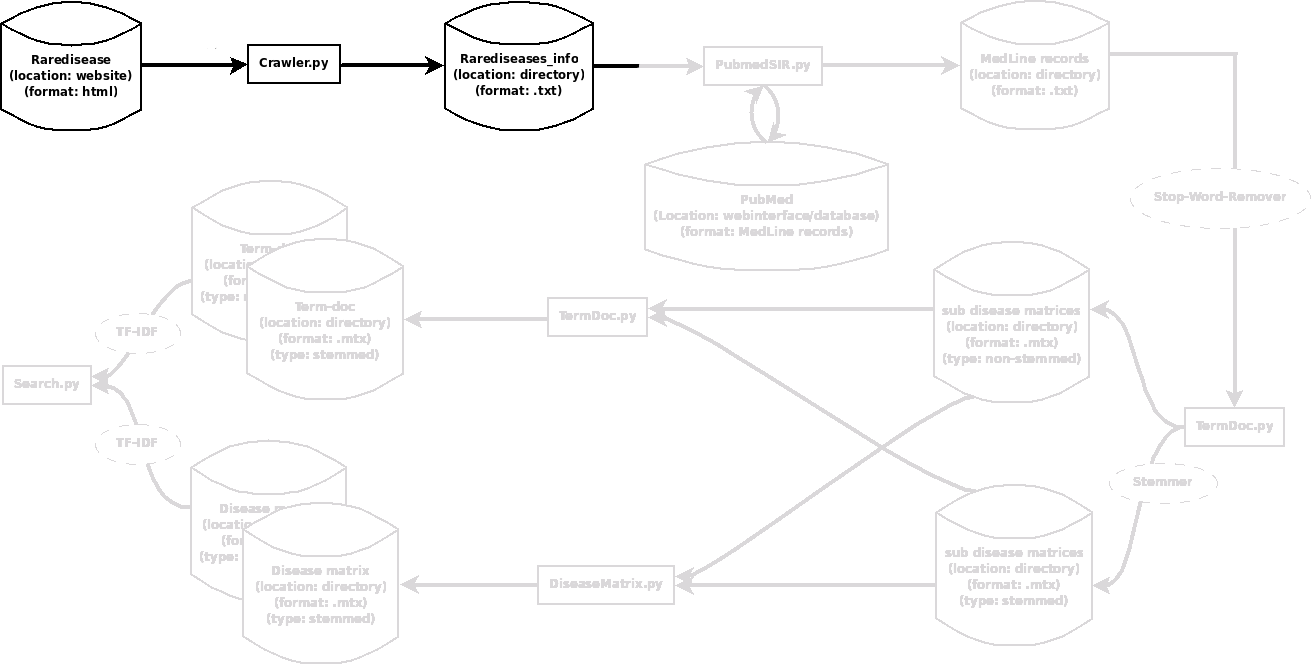
\includegraphics[width=1.0\textwidth]{diagram/system_overview1}}
    \only<2>{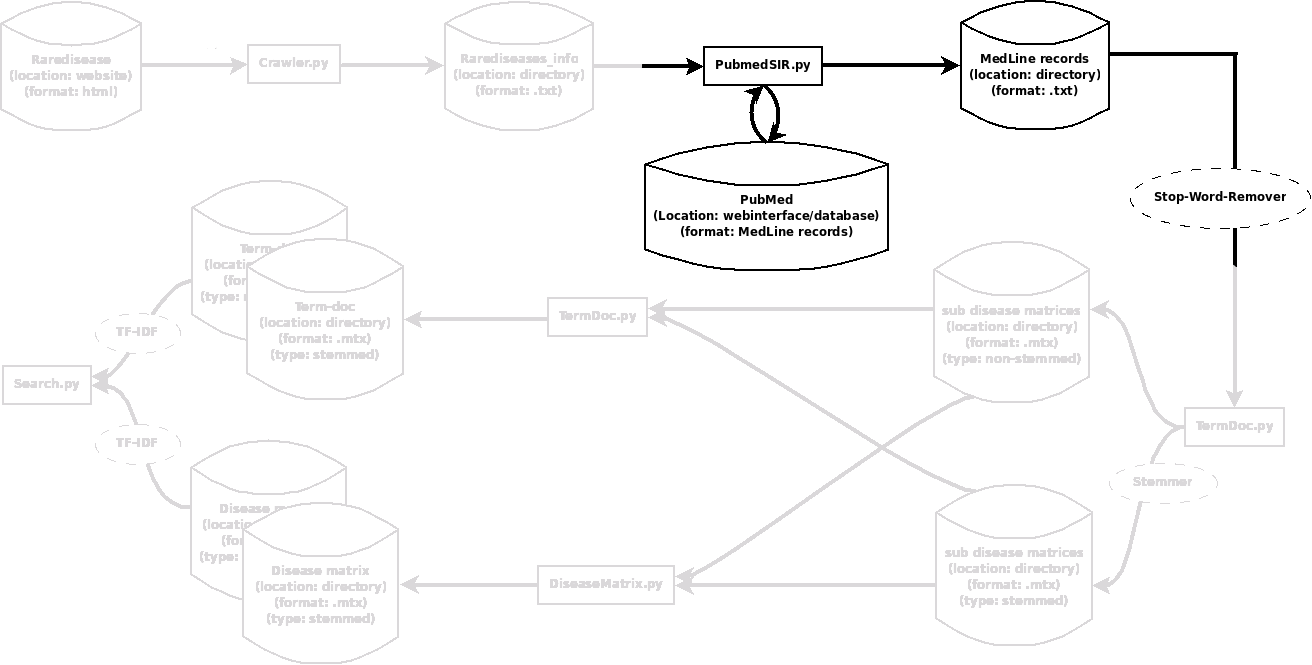
\includegraphics[width=1.0\textwidth]{diagram/system_overview2}}
    \only<3>{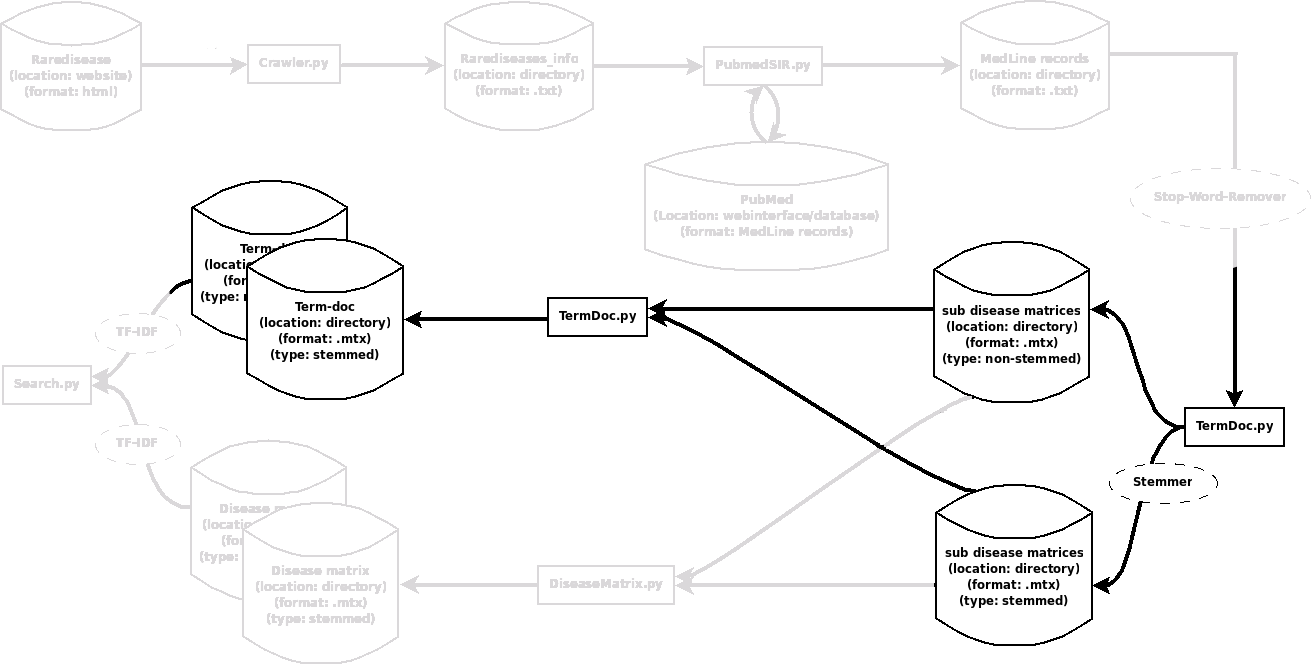
\includegraphics[width=1.0\textwidth]{diagram/system_overview3}}
    \only<4>{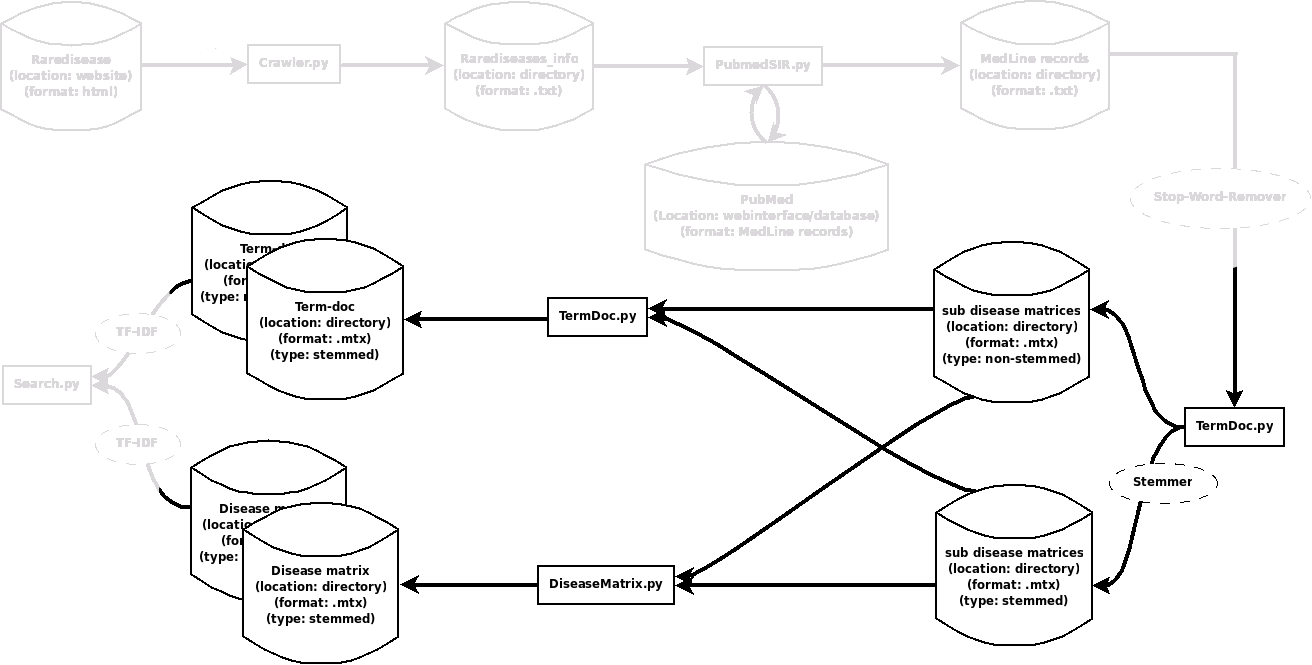
\includegraphics[width=1.0\textwidth]{diagram/system_overview4}}
    \only<5>{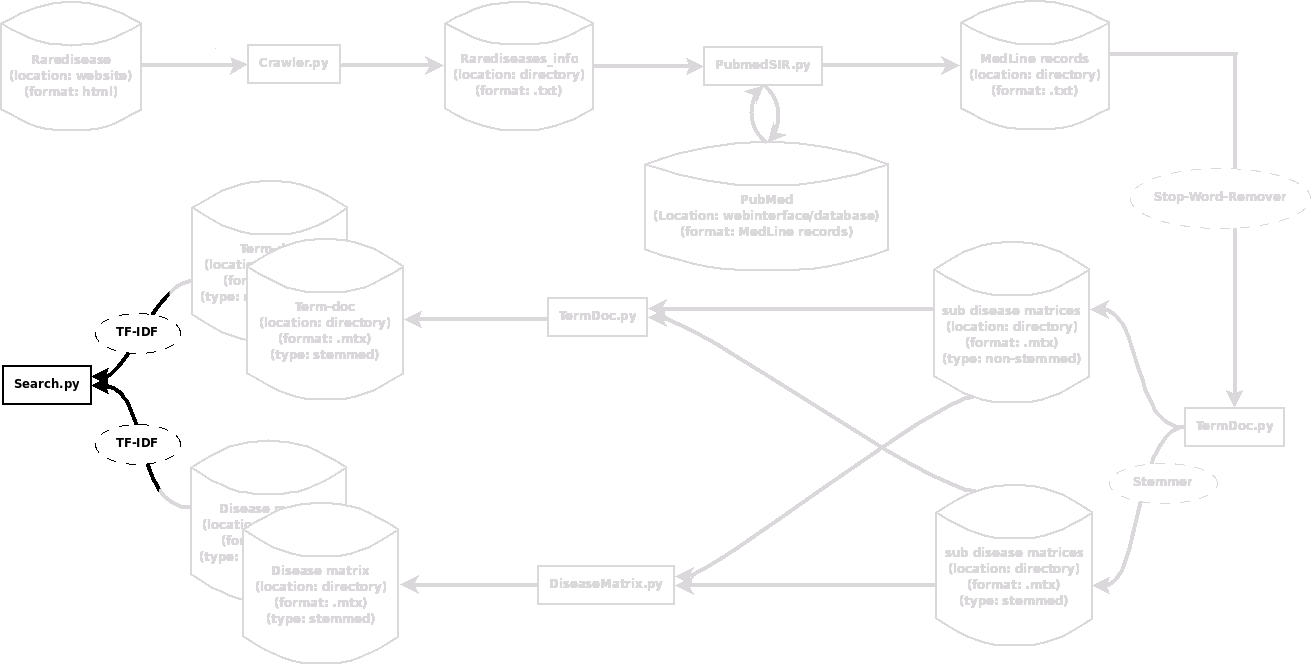
\includegraphics[width=1.0\textwidth]{diagram/system_overview5}}
    \only<6>{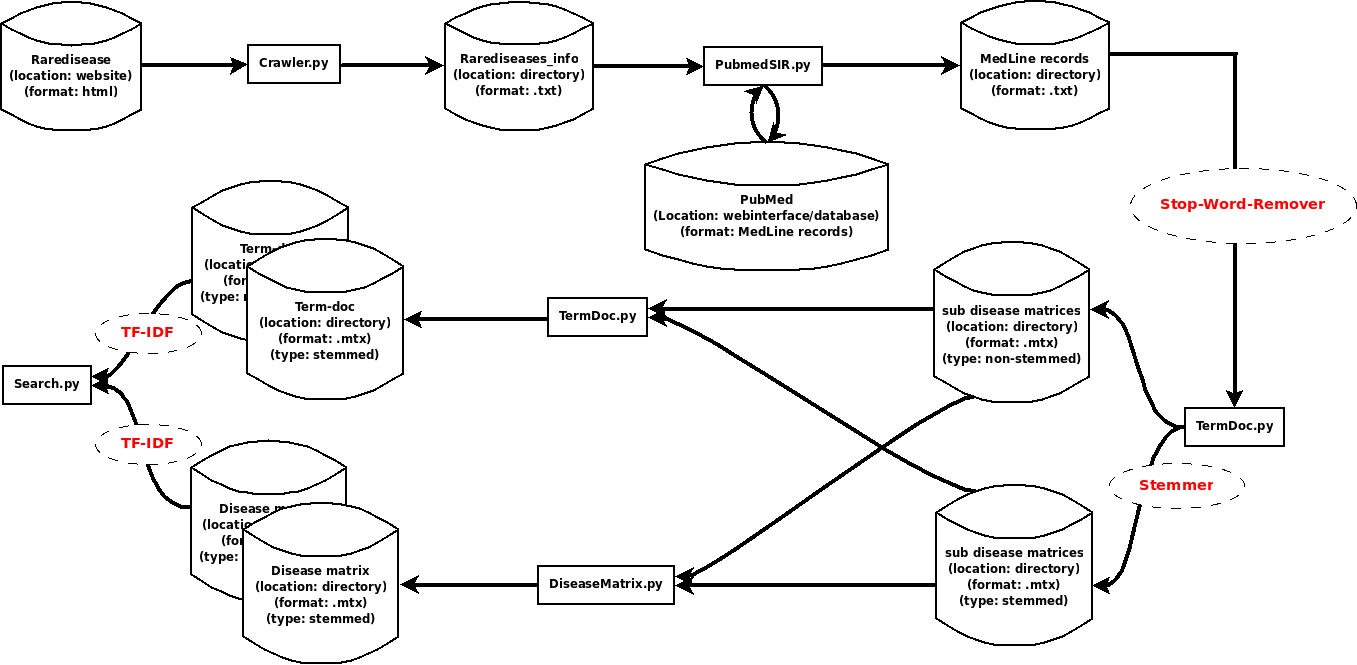
\includegraphics[width=1.0\textwidth]{diagram/system_overview6}}
    \only<7>{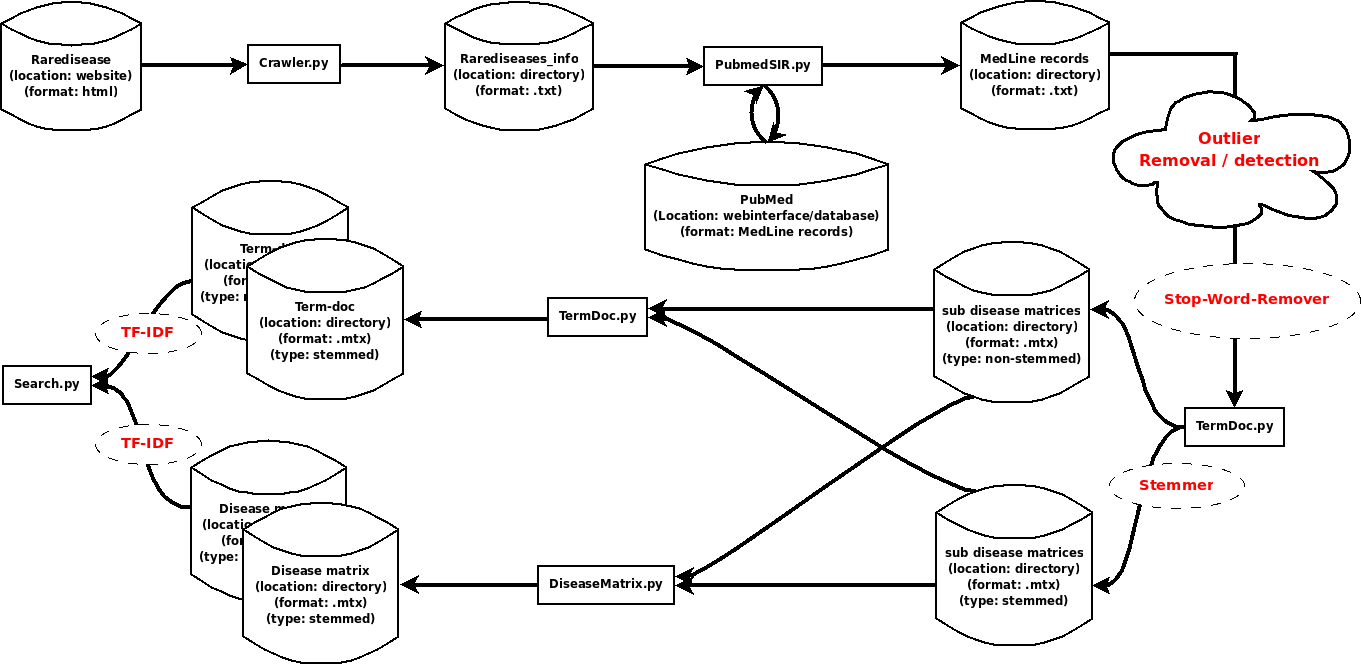
\includegraphics[width=1.0\textwidth]{diagram/system_overview7}}
    \only<8>{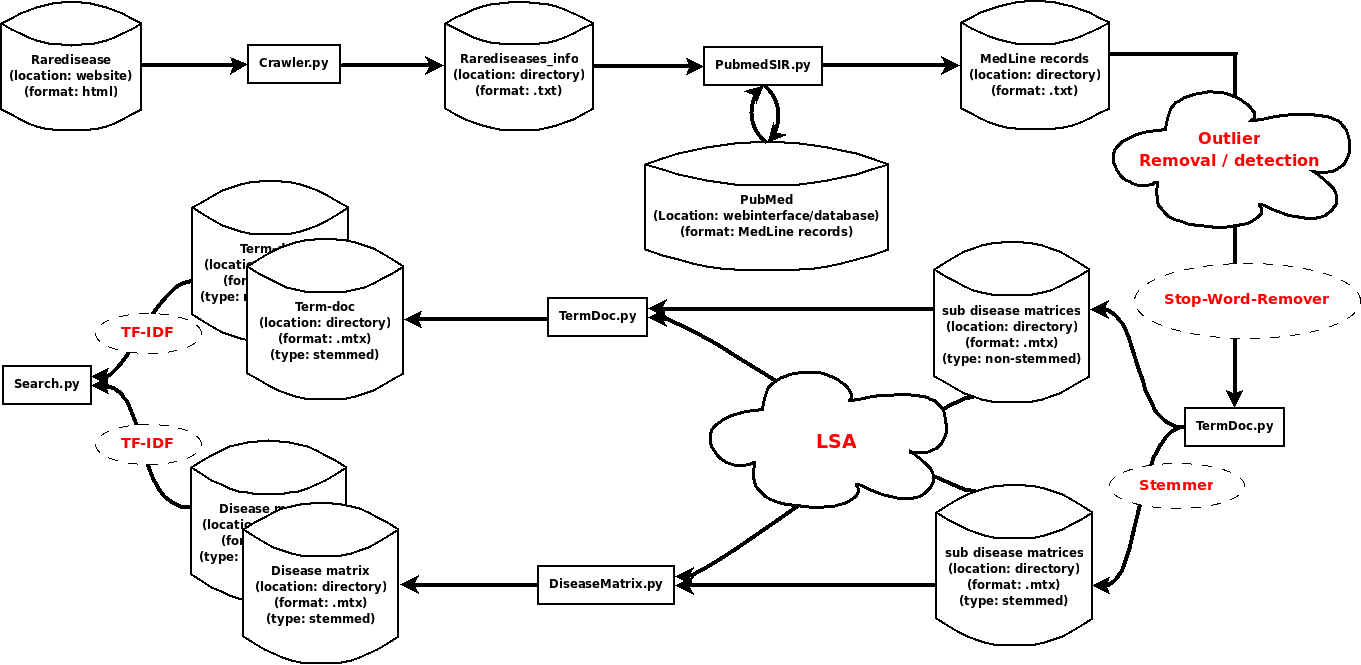
\includegraphics[width=1.0\textwidth]{diagram/system_overview8}}
    \only<9>{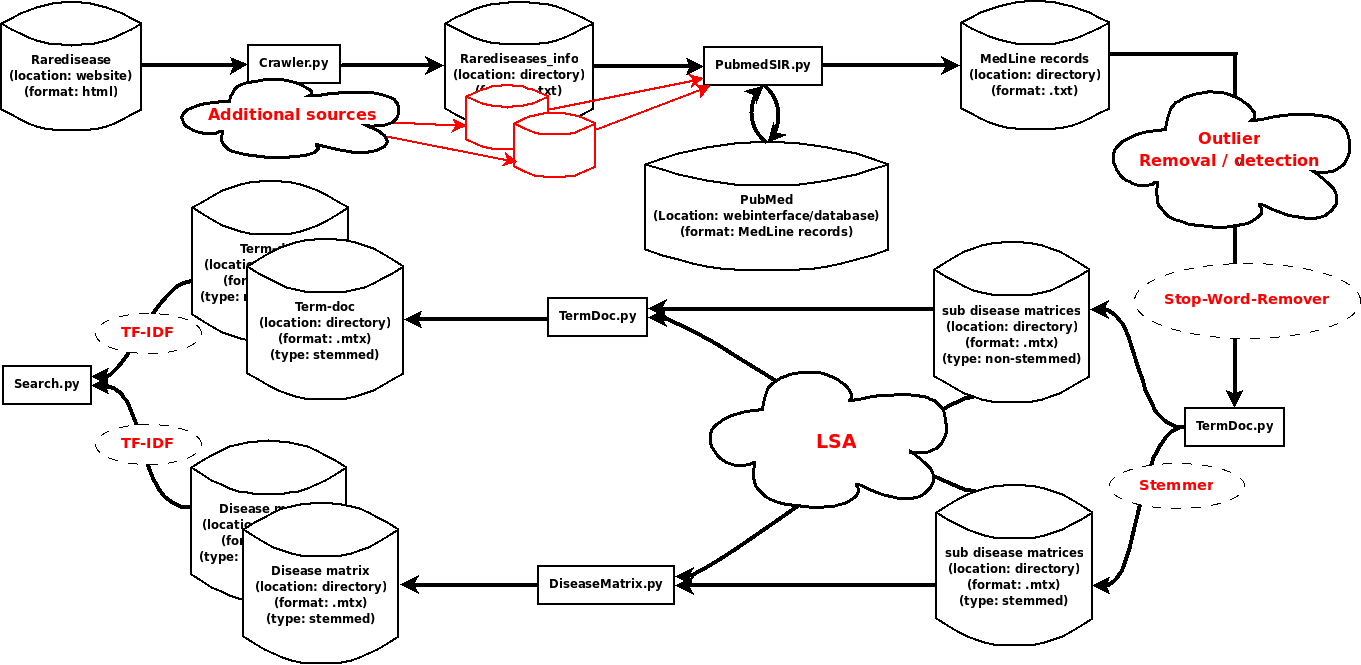
\includegraphics[width=1.0\textwidth]{diagram/system_overview9}}    
  \end{center}

\end{frame}

%% \begin{frame}

%%   \frametitle{Konstruktion af databasen}

%%   Inds\ae t tegning af interaktion mellem vores system og rarediseases, samt vores system og pubmed, endende med Medline Records.

%%   (evt. se figur 2.2 side 17)

%% \end{frame}

\begin{frame}

  \frametitle{Vector space model - Term doc matrix}

  \begin{center}
    \only<1>{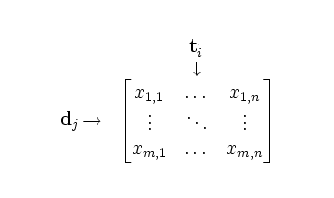
\includegraphics[width=0.65\textwidth]{diagram/termdoc1}}
    \only<2>{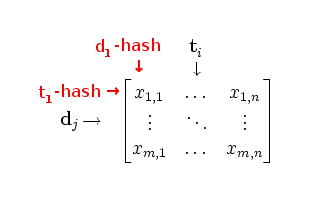
\includegraphics[width=0.65\textwidth]{diagram/termdoc2}}
  \end{center}

  $d_j$ hvor er en transponeret s\o jle vektor og $t_i$ er en term vektor.

\end{frame}

\begin{frame}

  \frametitle{V\ae gtning af term}

  Log-transformation af ord antallet:

  \[
  x_{dw}^{log} = \log{(1 + x_{dw})}
  \]

  Der bruges TF-IDF til v\ae gtning af termer, dette er for at fremh\ae ve term som sj\ae lendt optr\ae der og nedv\ae gte ofte forekommende ord:

  \[
  x_{dw}^{tfidf} = x_{dw}^{log} \cdot \log{\frac{D}{\sum_{d\prime = 1}^{D}\delta_{d\prime w}}}
  \]

  Afslutningsvis normaliseres dokument vektoren for at sikre de har ens indflydelse p\aa\ s\o geresultatet:

  \[
  x_{dw}^{norm} = \frac{x_{dw}^{tfidf}}{\sqrt{\sum_{w\prime = 1}^{W} {x_{dw}^{tfidf}}^{2}}}
  \]

\end{frame}

\begin{frame}

  \frametitle{Vector space model - Cosine score}

  Udregning af vinkel mellem en symptom liste og et dokument:
  
  \[
  \cos \theta_{D_d} = \frac{Q \circ D_d}{|Q| \cdot |D_d|}
  \]
  
  Ovenst\aa ende svarer til:
  
  \[
  \textrm{score}_{D_d} = \frac{1}{|I|}\frac{1}{|x_{dw}|} \sum_{i \in I} x_{dw}
  \]
  
  Hvis der p\aa\ forh\aa nd er foretaget normalisering af dokument vektoren:
  
  \[
  \propto  \sum_{i \in I} \widehat{x_{dw}}
  \]
  
\end{frame}

\begin{frame}

  \frametitle{Udregning af score for en sygdom}
  Score for sygdom j:
  $\textrm{disease}_j = \{\textrm{d}_1, \textrm{d}_2,
  \textrm{d}_3, \textrm{d}_4 \}$, hvor $d_i$ er dokument $i$.

  \begin{itemize}
    \item Cosine Median
      \begin{itemize}
        \item $ \textrm{disease}_j =
        \{\textrm{d}_1, \only<1>{\textrm{d}_2}
        \only<2->{\textbf{d}_{\mathbf{2}}}, \textrm{d}_3,
        \textrm{d}_{4} \}$
      \end{itemize}
    \item Cosine Max
      \begin{itemize}
        \item $ \textrm{disease}_j =
        \{\textrm{d}_{1}, \textrm{d}_{2},
        \textrm{d}_{3}, \only<1-2>{\textrm{d}_{4}}
        \only<3->{\textbf{d}_{\mathbf{4}}} \}$
      \end{itemize}
    \item Cosine ``Mean'' (Sum normaliseret)
      \begin{itemize}
        \item $\textrm{disease}_j = \sum_{i \in I} \{\textrm{d}_1,
          \textrm{d}_2, \textrm{d}_3, \textrm{d}_4 \}$
      \end{itemize}
    \item Sum unormaliseret (P\aa\ disease matrix)
      \begin{itemize}
        \item $\textrm{disease}_j = \sum_{i \in I} \widetilde{x_{dw}}$
      \end{itemize}
  \end{itemize}

\end{frame}

\section{Resultater}

\subsection*{}

\begin{frame}

  \frametitle{Diagnosticering af Sygdomme}

  \begin{itemize}
    \visible<1->\item Hvordan testes systemet? Eksempler:
  \end{itemize}

  \visible<2->{
  \begin{tabular}{|l|p{5cm}|}
    \hline
    Infective endocarditis & Acute, aortic, regurgitation, depression,
    abscess \\
    \hline
  \end{tabular}
  }
  
  \hspace*{4mm}

  \visible<3->{
  \begin{tabular}{|l|p{5cm}|}
    \hline
    Cholera \quad & severe diarrhea and vomiting \\
    \hline
  \end{tabular}
  }

  \hspace*{4mm}

  \visible<4->{
  \begin{tabular}{|l|p{5cm}|}
    \hline
    Kleine Levin Syndrome & Jewish boy age 16, monthly seizures, sleep
    deficiency, aggressive and irritable when woken, highly increased
    sexual appetite and hunger \\
    \hline
  \end{tabular}
  }


\end{frame}

\begin{frame}

  \frametitle{BMJ Resultater}

  \begin{center}
    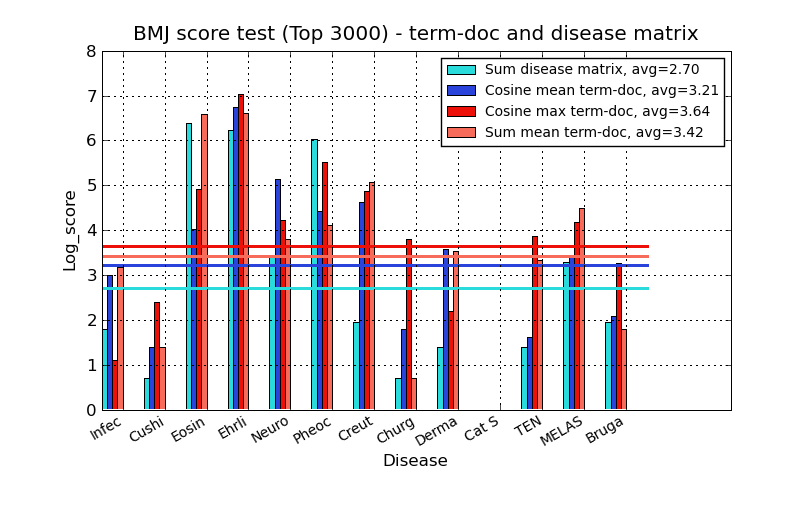
\includegraphics[width=1.0\textwidth]{diagram/termDoc_bmj_hist_3000_sum_dm_mea_cos_sqrt_td_max_cos_sqrt_td_mea_sum_td}
  \end{center}

\end{frame}

\begin{frame}

  \frametitle{Orpha.net Resultater}

  \begin{center}
    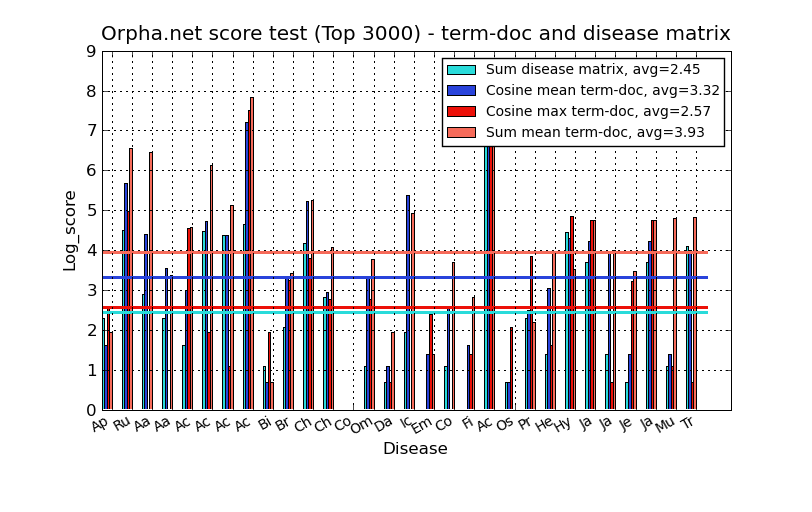
\includegraphics[width=1.0\textwidth]{diagram/termDoc_orphan_hist_3000_sum_dm_mea_cos_sqrt_td_max_cos_sqrt_td_mea_sum_nn_td}
  \end{center}

\end{frame}

\begin{frame}

  \frametitle{Blind tests Resultater}

  \begin{center}
    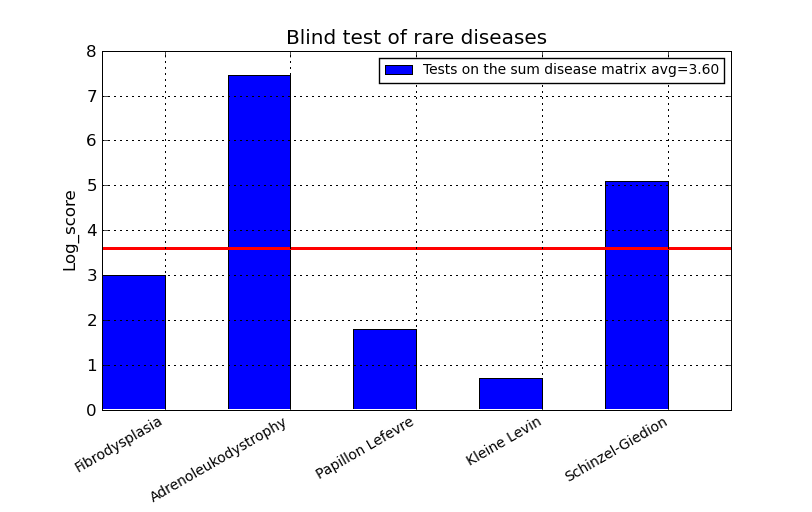
\includegraphics[width=1.0\textwidth]{diagram/blind_test}
  \end{center}

\end{frame}

\begin{frame}

  \frametitle{Forkerte forslag}

  Hvorfor rammer vi ikke den korrekte sygdom?

  \begin{table}[H]
    \begin{tiny}
      \begin{center}
        \begin{tabular}{|c|c|}
          \hline
          \scriptsize{\textbf{Adrenoleukodystrophy}} & \scriptsize{\textbf{Kleine Levin}} \\
          \hline
          pex26 &lein  \\
          \hline
          pex1 &megaphagia \\
          \hline
          pex13 &hypersomnia\\
          \hline
          pex5 &levin\\
          \hline
          nald &hypersomn\\
          \hline
          pts1 &kl\\
          \hline
          ldpex5 &hypersomniac\\
          \hline
          pex12 &hypersexu \\
          \hline
          pex5p &hypersomnol\\
          \hline
          peroxin&asmp \\
          \hline
          pex10 &narcolepsi\\
          \hline
          zs &hypocretin\\
          \hline
          pbd &mslt \\
          \hline
          pex14 &hyperphagia\\
          \hline
          g843d &pickwickian \\
          \hline
          pex12p &somnol\\
          \hline
          pex1p &ceretec\\
          \hline
          ird &parasomnia\\
          \hline
          pts1r &rem\\
          \hline
          pts2 &smp\\
          \hline
        \end{tabular}
      \end{center}
    \end{tiny}
  \end{table}
  
\end{frame}

\begin{frame}

  \frametitle{Forkerte forslag 2}
  \begin{itemize}
    \item\visible<1->{Sygdommen \emph{Acropectorovertebral dysplasia}'s information er baseret p\aa\ en MedLine Record.}

    \item\visible<2->{Der er brug for mere diversitet i termerne / flere synonymer for symptomer.}

    \item\visible<3->{Informationen er baseret p\aa\ h\o jest 500 MedLine Records.}
  \end{itemize}

\end{frame}

\begin{frame}

  \frametitle{Clustering af resultater}

  \begin{center}
     \only<1>{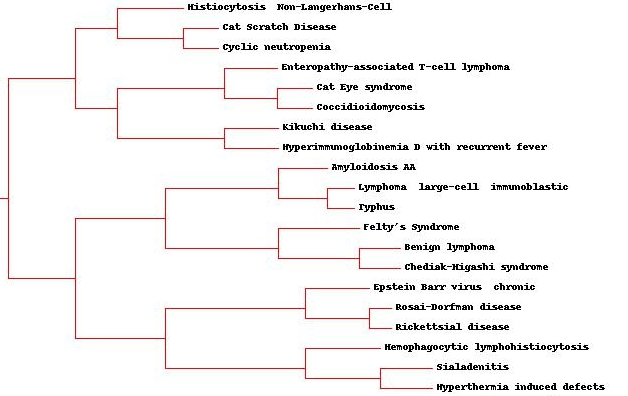
\includegraphics[width=0.90\textwidth]{diagram/cluster_cat_scratch.jpg}}
     \only<2>{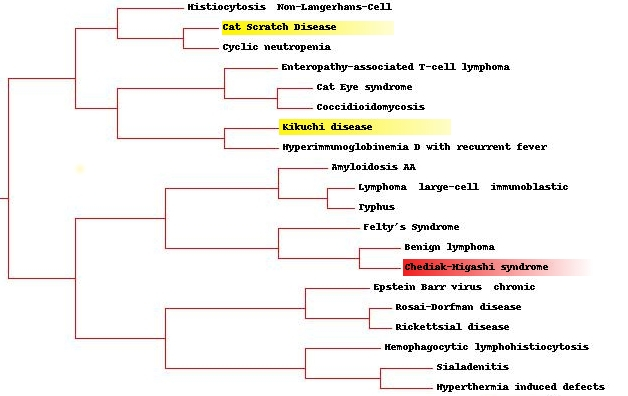
\includegraphics[width=0.90\textwidth]{diagram/cluster_cat_scratch2.jpg}}
  \end{center}

\end{frame}

\section{Fremtidige muligheder}

\subsection*{}

\begin{frame}

  \frametitle{Udvidelser}

  \begin{itemize}
    \item Statistisk model.
    \item Tilf\o jelse af andre heuristikker.
    \item Keyword extraction fra sygdomme.
    \item Udvidet mulighed for s\o gning, f.eks. sammenligning af s\o
      gninger, boolske operatorer.
  \end{itemize}

\end{frame}

\begin{frame}

  \frametitle{Outlier detection}

  Afstandsmatrix hvor cosine er brugt som afstandsm\aa l. Sidste s\o
  jle beskriver Mean Distance To Others.

%  \begin{multicols}{2}
  \begin{center}
    \begin{tabular}{|l|r|r|r|r|r|}
      \hline
      DM    & d$_1$ & d$_2$ & d$_3$ & d$_4$ & MDTO \\
      \hline
      d$_1$ &   1.0 &   0.3 &   0.7 &   0.8 & 0.7 \\
      \hline
      d$_2$ &   0.3 &   1.0 &   0.5 &   0.6 & 0.6 \\
      \hline
      d$_3$ &   0.7 &   0.5 &   1.0 &   0.3 & 0.625 \\
      \hline
      d$_4$ &   0.8 &   0.6 &   0.3 &   1.0 & 0.675 \\
      \hline
    \end{tabular}
  \end{center}

%  \end{multicols}

  Andre metoder, f.eks. afstand fra middel vektor, K-means
  clustering.

\end{frame}

\section{Konklusion}

\begin{frame}

  \frametitle{Konklusion}

  \begin{itemize}
    \visible<1->{\item Andre transformation b\o r afpr\o ves}
    \visible<2->{\item Rammer omkring 60\%}
    \visible<3->{\item Minimum gr\ae nse for information per sygdom}
    \visible<4->{\item St\o j reduktion n\o dvendigt}
    \visible<5->{\item Medicinsk dom\ae ne viden n\o dvendigt}
  \end{itemize}

  \hspace*{1cm}

%  \begin{center}
  \visible<6>{\textbf{Tak!}}
%  \end{center}

\end{frame}

\end{document}
